\subsection{子空间的商空间}

设 X 是拓扑空间，A 是 X 的一个子空间，R 是 X 上的一个等价关系，f 是典范映射 \(X \to X/R\)，g 是 f 在 A 上的限制。A 上的等价关系 \(g(x) = g(y)\) 恰是 R 在 A 上诱导的关系 \(R_{A}\)（《集合论》R，§ 5，第 5 目）。设 \(g = \psi \circ h \circ \varphi\) 是 g 的典范分解，于是若 j 是 A 到 X 中的典范单射，我们就有一个交换图 (*)

\begin{enumerate}
\def\labelenumi{(\Roman{enumi})}
\tightlist
\item
\end{enumerate}

\pandocbounded{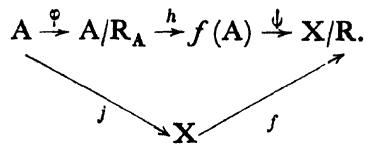
\includegraphics[keepaspectratio]{images/part001_6dc64900.jpg}}

命题 10. 典范双射 \(h: \mathbf{A} / \mathbf{R}_{\mathbf{A}} \to f(\mathbf{A})\) 是连续的。此外，下列三个命题等价：

\begin{enumerate}
\def\labelenumi{\alph{enumi})}
\item
  \(h\) 是一个同胚。
\item
  A 的每个关于 \(R_{A}\) 饱和的开子集都是 X 的某个关于 R 饱和的开子集与 A 的交。
\item
  A 的每个关于 \(R_{A}\) 饱和的闭子集都是 X 的某个关于 R 饱和的闭子集与 A 的交。
\end{enumerate}

命题的第一部分是直接的（第 5 目）。第二部分由第 5 目命题 8 得出：若 B 是 A 的关于 \(R_{A}\) 饱和的开（相应地，闭）子集，且 \(g(B) = f(B)\) 是 X/R 的某个开（相应地，闭）子集 C 与 \(f(A)\) 的交，则 B 是开（相应地，闭）子集 \(\overline{f}(C)\)

与 A 的交，该子集关于 R 饱和；反之，若 B 是某个关于 R 饱和的开（相应地，闭）子集 D 与 A 的交，则 \(f(\mathbf{B})\) 是 \(f(\mathbf{A})\) 与 \(f(\mathbf{D})\) 的交，而它在 X/R 中是开（相应地，闭）集。

推论 1. 若 A 是 X 的关于 R 饱和的开（相应地，闭）子集，则典范映射 \(h: \mathrm{A}/\mathrm{R}_{\mathrm{A}} \rightarrow f(\mathrm{A})\) 是一个同胚。

因为若 A 在 X 中开（相应地，闭）且关于 R 饱和，且 \(B \subset A\) 在 A 中开（相应地，闭）且关于 \(R_{A}\) 饱和，则 B 在 X 中开（相应地，闭）且关于 R 饱和。

推论 2. 若存在连续映射 \(u: \mathbf{X} \to \mathbf{A}\)，使得 \(u(x)\) 与 \(x \mod \mathbb{R}\) 同余（对每个 \(x \in \mathbf{X}\)），则 \(f(\mathbf{A}) = \mathbf{X} / \mathbb{R}\)，且典范映射 \(h: \mathbf{A} / \mathbb{R}_{\mathbf{A}} \to \mathbf{X} / \mathbb{R}\) 是一个同胚。

由于模 R 的每个等价类都与 A 相交，\(A/R_{A}\) 在 X/R 中的典范像是整个 X/R；另一方面，若 U 在 A 中开且关于 \(R_{A}\) 饱和，则由假设可知，\(\overline{u}^{1}(U)\) 是把 U 关于 R 饱和化所得到的集合；由于 u 连续，\(\overline{u}^{1}(U)\) 在 X 中是开集（§ 2，第 1 目，定理 1）。由这一事实并借助命题 10 即得推论。

例。* 设 R 表示实直线 R 上的等价关系 \(x \equiv y \pmod{1}\)（第 4 目，例），且设 A 表示闭区间 {[}0, 1{]}；A 包含模 R 每个等价类的至少一个点。\(\mathrm{A} / \mathbb{R}_{\mathbf{A}}\) 到环面 T 上的典范映射是一个同胚；因为若 F 在 A 中闭（从而在 R 中闭），则为把 F 关于关系 R 饱和化，须取诸闭集 \(\mathrm{F} + n\)（对所有 \(n \in \mathbf{Z}\)）的并，它们显然构成一个局部有限族，故其并是闭集（§ 1，第 5 目，命题 4）；断言由此得出。我们指出，\(\mathrm{A} / \mathbb{R}_{\mathbf{A}}\) 是把 A 中的点 0 与 1 等同起来得到的。*

